\documentclass[utf8]{ctexart}
\usepackage{graphicx}
\usepackage{amsmath,amssymb,amsthm}
\usepackage{geometry}
\usepackage{enumitem}
\usepackage{xcolor}
\usepackage{mdframed}
\usepackage{tikz}
\usepackage{booktabs,array}
\usepackage{needspace}
\usepackage[hidelinks]{hyperref}
\usetikzlibrary{arrows.meta,positioning,calc}
\geometry{a4paper,margin=2.5cm}

\newtheoremstyle{mystyle}
  {8pt}{8pt}{\kaishu}{0pt}{\bfseries}{}{1em}{}
\theoremstyle{mystyle}
\newtheorem{theorem}{定理}
\newtheorem{lemma}{引理}

\title{\textbf{人工智能导论\quad 第一次作业}}
\date{\today}
\author{李子嘉 2024012325}

\begin{document}
\maketitle

\section*{题目1}
\textbf{证明：}

当终点 $T$ 即将从边缘集（frontier）中取出时，树搜索的边缘集中仍有
最优路径上的某个节点 $n^*$，其对应路径为该最优路径的前缀，因而
\[
  g(n^*)+h^*(n^*)=h^*(S).
\]
由于 $T$ 的 $f$ 值最小，且 $h(T)=0$，故
\[
  g(T)=f(T)\le f(n^*)=g(n^*)+h(n^*).
\]

\subsection*{（1）}
代入 $h(n^*)\le h^*(n^*)+C_1$，得到
\[
  g(T)\le g(n^*)+h^*(n^*)+C_1=h^*(S)+C_1.
\]

\subsection*{（2）}
由边代价非负可知 $g(n^*)\ge0$，又有 $C_2\ge1$，因此
\begin{align*}
  g(T)
  &\le g(n^*)+C_2h^*(n^*)\\
  &\le C_2\bigl(g(n^*)+h^*(n^*)\bigr)
   =C_2h^*(S).
\end{align*}

\newpage
\subsection*{（3）}
记最优代价为 $C^*=h^*(S)$，返回解的代价为 $C=g(T)$。
这里先考虑不重新打开 CLOSED 节点的图搜索，仍更新 OPEN 中的更优路径，
按 $g+h$ 取出节点，并在取出终点时停止。

\medskip
\noindent\textbf{先检查不高估的情形。}
看到“类似的结论”，我首先想到沿用前两问的条件。但不妨先令 $C_1=0$
或 $C_2=1$：此时条件都是 $h\le h^*$，结论都应当退化为 $C=C^*$。
而我们知道，不重新打开节点的图搜索仅靠不高估并不能保证最优，
还可能因为不一致的启发函数过早关闭节点。因此，我们猜测这种直接推广并不成立，
并用下面的例子确认这一点：
\begin{center}
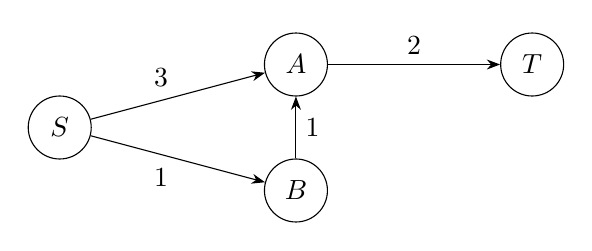
\begin{tikzpicture}[
  >=Stealth,
  vertex/.style={circle,draw,minimum size=8mm,inner sep=0pt},
  every edge/.style={draw,->},
  every edge quotes/.style={fill=white}
]
  \node[vertex] (S) at (0,0) {$S$};
  \node[vertex] (A) at (3,0.8) {$A$};
  \node[vertex] (B) at (3,-0.8) {$B$};
  \node[vertex] (T) at (6,0.8) {$T$};
  \draw[->] (S) -- node[above left] {$3$} (A);
  \draw[->] (S) -- node[below left] {$1$} (B);
  \draw[->] (B) -- node[right] {$1$} (A);
  \draw[->] (A) -- node[above] {$2$} (T);
\end{tikzpicture}
\end{center}
按 $S,A,B,T$ 的顺序取
\[
 (h(S),h(A),h(B),h(T))=(4,0,3,0),\qquad
 (h^*(S),h^*(A),h^*(B),h^*(T))=(4,2,3,0).
\]
扩展 $S$ 后，$f(A)=3<f(B)=4$，所以先关闭 $A$，生成 $g(T)=5$。
随后扩展 $B$，发现代价为 $2$ 的路径 $S\to B\to A$，但不再打开 $A$，
最终返回 $C=5$；最优路径 $S\to B\to A\to T$ 的代价却是 $C^*=4$。
这里所有节点均满足 $h\le h^*$，但 $h(B)=3>1+h(A)$，违反了一致性。

这说明连不高估的基准情形都不能保证最优，因而已经没有必要再尝试证明
原条件对一般 $C_1,C_2$ 的机械推广。联想到图搜索的问题并不只是启发函数是否高估，而在于 CLOSED 节点不再打开，因此更自然的量是启发函数违反一致性的程度。于是我们思考：
\textbf{如果放宽的是一致性条件，能否得到类似的误差控制？}

\medskip
\noindent\textbf{带着这个问题查阅文献。}
我们检索后发现，Valenzano 等人\cite{valenzano2014}恰好研究了不重新展开节点时的
解质量损失。以下按文献取有限图、有限非负启发函数、非负边代价及 $h(T)=0$，
用每条边对一致性条件的违反程度
\[
 I(u,v)=\max\{h(u)-c(u,v)-h(v),\,0\}.
\]
来度量误差。设 $P^*=(n_0=S,n_1,\ldots,n_k=T)$ 为最优路径，$k\ge1$，
该文定理 4.6 给出
\begin{equation}
 \boxed{C\le C^*+\sum_{j=1}^{k-1}I(n_j,n_{j+1}).}
 \label{eq:inconsistency-bound}
\end{equation}
这个结论不要求 $h$ 不高估。求和不含首边，因为 $S$ 首先以正确的 $g(S)=0$
扩展，最优路径上的 $n_1$ 会获得正确的前缀代价。

为了看清它与前两问的联系，我们整理证明的关键步骤。在取出 $T$ 前，选 $P^*$ 上最靠近起点的
OPEN 节点 $n_i$，则
\[
 C\le f(n_i)
 =C^*+\underbrace{g(n_i)-g^*(n_i)}_{\text{前缀代价误差}}
       +\underbrace{h(n_i)-h^*(n_i)}_{\text{启发估计误差}}.
\]
文献的定理 4.5 及其对该 OPEN 节点的推论给出前缀误差界；
后缀误差界则由 $h(n_j)-h(n_{j+1})-c(n_j,n_{j+1})\le I(n_j,n_{j+1})$
沿后缀求和得到：
\[
 g(n_i)-g^*(n_i)\le\sum_{j=1}^{i-1}I(n_j,n_{j+1}),\qquad
 h(n_i)-h^*(n_i)\le\sum_{j=i}^{k-1}I(n_j,n_{j+1}).
\]
两式相加即得式\eqref{eq:inconsistency-bound}。相比前两问，这里多出的 $g$ 值误差
也由不一致量控制，其中前缀误差的归纳结论引用自文献。

\newpage
\noindent\textbf{回到本题，尝试给出相应的条件。}
有了式\eqref{eq:inconsistency-bound}，我们就可以从一致性出发，分别尝试加法和乘法放宽，
并直接证明与前两问对应的结论。
\begin{enumerate}[label=\arabic*.,leftmargin=2em,itemsep=8pt]
 \item \textbf{加法放宽：}
 若每条边都有 $h(u)\le c(u,v)+h(v)+\delta$，其中 $\delta\ge0$，则
 \[
   I(u,v)\le\delta
   \quad\Longrightarrow\quad C\le C^*+(k-1)\delta.
 \]
 若已知最优路径至多有 $D$ 条边，则可用 $(D-1)\delta$ 作统一加法误差界。
 与第（1）问不同，每条边的放宽量会累积；若希望仍保证 $C\le C^*+C_1$，
 一个充分条件是最优路径上除首边外的不一致量之和不超过 $C_1$。

 \item \textbf{乘法放宽：}
 若每条边都有 $h(u)\le w\,c(u,v)+h(v)$，其中 $w\ge1$，则
 \[
   I(u,v)\le(w-1)c(u,v),
   \qquad
   C\le C^*+(w-1)\sum_{j=1}^{k-1}c(n_j,n_{j+1})\le wC^*.
 \]
 取 $w=C_2$ 就得到与第（2）问相同形式的界，但条件从点上的
 $h\le C_2h^*$ 加强为每条边上的不等式。
\end{enumerate}

\medskip
\noindent\textbf{结论}
所以图搜索确实存在与前两问类似的误差界，但需要控制的是一致性误差而不是单个节点上的高估误差，且加法放宽的程度与最优路径的长度有关，不好控制。若允许重新打开 CLOSED 节点，则原来的 admissibility 型条件又可以得到相应的界。

\begingroup
\small
\begin{thebibliography}{9}
\bibitem{valenzano2014}
R. Valenzano, N. R. Sturtevant, and J. Schaeffer.
\href{https://www.cs.du.edu/~sturtevant/papers/non_reopening.pdf}
{Worst-Case Solution Quality Analysis When Not Re-Expanding Nodes in Best-First Search}.
AAAI, 2014. 第 4.1--4.3 节，尤其定理 4.5、4.6。
\end{thebibliography}
\endgroup

% 后续题目继续使用 \section*{题目2} 等标题。
% 第二题按要求将本人学号题组的“答案正确”截图插入统一报告，无须另写逐步推导。
% 完成最终报告时，请自行调整文字，并按题面要求在末尾声明大模型辅助的方式和程度。（帮助查阅第一题第三问的开放式问题相关文献并总结定理证明）

\end{document}
